%====================================================================================
\section[Coase]{Teorema de Coase}
%====================================================================================

\begin{frame}{Teorema de Coase}
	\begin{itemize}
		\item El llamado ``Teorema de Coase'' propone que los agentes económicos resolverán los problemas de externalidad sin intervención.
		\item El Teorema puede formularse como:
			\emph{``En una econpmía competitiva, con información completa y costos de transacción nulos, la asignación de recursos será eficiente e invariable con respecto a las reglas legales de titularidad''}.
		\item Las reglas legales de titularidad (o \emph{derechos de propiedad}) determinan la propiedad en la economía.
		\item Coase ve las externalidades como surgidas por la ausencia de derechos de propiedad
			\begin{itemize}
				\item La contaminación ocurre cuando no hay derecho a aire limpio o agua limpia.
			\end{itemize}
		\item Si hubiera un derecho de propiedad, cualquiera que sufra una externalidad recibiría una compensación.
		\item La compensación es el precio por la externalidad.
		\item El intercambio competitivo asegura que surja el precio correcto y que se alcance la eficiencia.
	\end{itemize}
\end{frame}
%------------------------------------------------
\begin{frame}{Teorema de Coase}
	\begin{itemize}
		\item Coase ve las externalidades como surgidas por la ausencia de derechos de propiedad
			\begin{itemize}
				\item La contaminación ocurre cuando no hay derecho a aire limpio o agua limpia.
			\end{itemize}
		\item Si hubiera un derecho de propiedad, cualquiera que sufra una externalidad recibiría una compensación.
		\item La compensación es el precio por la externalidad.
		\item El intercambio competitivo asegura que surja el precio correcto y que se alcance la eficiencia.
		\item El Teorema también afirma que el equilibrio es invariable a la asignación de derechos de propiedad.
		\item Una empresa, ¿contaminará la atmósfera de una casa vecina?
			\begin{itemize}
				\item Sólo si el beneficio de hacerlo excede la compensación requerida por el propietario de la casa.
				\item Esto se aplica si la empresa tiene el derecho a contaminar o si el propietario de la casa tienenel derecho a aire limpio.
			\end{itemize}
	\end{itemize}
\end{frame}
%------------------------------------------------
\begin{frame}{Teorema de Coase}
	\begin{itemize}
		\item La distribución final de ingreso será diferente.
		\item El equilibrio no cambiará por la asignación de derechos de propiedad si no hay efectos ingreso.
		\item Las limitaciones prácticas del Teorema de Coase son:
			\begin{itemize}
				\item La carencia de derechos de propiedad claros.
				\item Los costos de transacción en alcanzar acuerdos de compensación
				\item Las implicancias de la negociación bilateral y la ineficiencia potencial con información incompleta.
				\item El poder de monopolio potencial.
			\end{itemize}
		\item El Teorema de Coase sugiere una resolución al problema de las externalidades pero hay razones por las cuales el mercado puede no funcionar.
	\end{itemize}
\end{frame}
%------------------------------------------------
\begin{frame}{Teorema de Coase}
	Volviendo al ejemplo:
		\begin{itemize}
			\item Supongamos que la piscigranja tenga derecho a tener agua pura, y lo vende para permitir que la suderurgia contamine.
			\item Sea $q$ el precio por unidad de contaminación.
		\end{itemize}
\end{frame}
%------------------------------------------------
\begin{frame}{Creación de mercados de derechos (Coase)}
	Los problemas de maximización serán:\\
		\begin{center}
			\begingroup
			\setlength{\tabcolsep}{10pt} % Default value: 6pt
			\renewcommand{\arraystretch}{1.5} % Default value: 1
				\begin{tabular}{ccc}
						\hline
					Para la acería & {} & Para la piscigranja\\
					$\M \limits_{s,x} \pi_s = p_ss - c_s(s,x) -qx$ & {} & $\M \limits_{f,x} \pi_f = p_f - c_f(f,x) +qx$\\
						\hline 
					\multicolumn{3}{c}{condiciones de primer orden} \\
					\hline
					$\frac{\partial \pi}{\partial s} = 0 \Leftrightarrow p_s - \frac{\partial c_s}{\partial s} = 0$ & {} & $\frac{\partial \pi}{\partial f} = 0 \Leftrightarrow p_f - \frac{\partial c_f}{\partial f} = 0$\\
					$p_s = \frac{\partial c_s}{\partial s}$ & {} & $p_f = \frac{\partial c_f}{\partial f}$\\
					$\frac{\partial \pi}{\partial x} = 0 \Leftrightarrow - \frac{\partial c_s}{\partial x} - q = 0$ &{} & 	$\frac{\partial \pi}{\partial x} = 0 \Leftrightarrow - \frac{\partial c_f}{\partial x} + q = 0$\\
					$q = -\frac{\partial c_s}{\partial x}$& {} & $q = \frac{\partial c_f}{\partial x}$ \\
						\hline
				\end{tabular}
			\endgroup
		\end{center}
	En consecuencia, se llega a las condiciones de eficiencia:
		$$-\frac{\partial c_s}{\partial x}=\frac{\partial c_f}{\partial x}$$
\end{frame}
%------------------------------------------------
\begin{frame}{Equilibrio general competitivo y externalidad negativa}
	\begin{center}
		\includegraphics[width = 1\linewidth]{figures/equilibrio.pdf}
	\end{center}
\end{frame}

%------------------------------------------------------------------------------------
\subsection{Más sobre el Teorema de Coase}
%------------------------------------------------------------------------------------
\begin{frame}{Más sobre el Teorema de Coase}
Ejemplo del panadero y del médico:
	\begin{itemize}
		\item La máquina del panadero produce ruido y vibraciones que molestan a un médico vecino.
		\item Evitar el daño al médico implica infligir daño al panadero.
		\item Problema de fondo: ¿vale la pena reducir la producción de dulces para aumentar la de servicios médicos?
		\item El médico demandó al panadero y la corte le dio la razón.
		\item Pero para Coase, el médico habría aceptado que siga funcionando la máquina del panadero, si el panadero hubiere pagado una suma mayor a la pérdida del médico.
	\end{itemize}	
\end{frame}
%------------------------------------------------
\begin{frame}{Más sobre el Teorema de Coase}
Ejemplo del panadero y del médico:
	\begin{itemize}
		\item Igual, el panadero habría aceptado pagar un monto menor a su pérdida por el cambio o reducción de su nivel de producción.
		\item Según Coase, la solución sólo dependía de si el uso continuo de la maquinaria añade al ingreso del panadero más de lo que resta al ingreso del doctor.
		\item Si ambos hubiesen llegado a un acuerdo sin mayor costo, la decisión de cuál mantenía su actividad dependía de los ingresos involucrados.
		\item En consecuencia, la decisión del juez era irrelevante.
	\end{itemize}
\end{frame}
%------------------------------------------------
\begin{frame}{Gráficamente}
	\begin{multicols}{2}
		\begin{itemize}
			\item $BMNP$= Beneficio Marginal Neto Privado = beneficio adicional que obtiene la panadería por unidad producida.
			\item $DM$ = Daño Marginal = perjuicio adicional que la panadería provoca al médico.
		\end{itemize}
		
		\begin{center}
			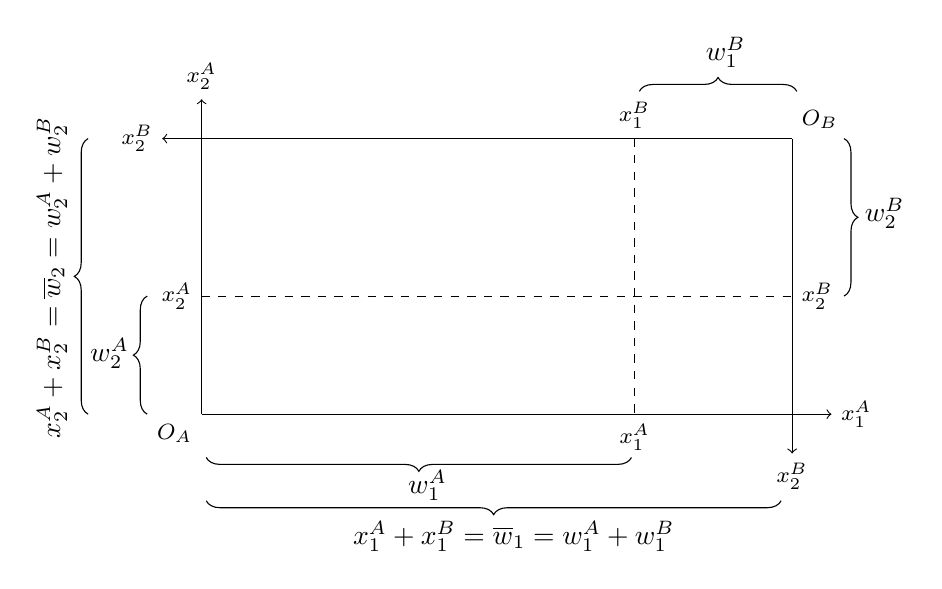
\begin{tikzpicture}[scale=1]
	% Formación de la caja
		% Consumidor A
			\draw[->] (0.5,0.5) node[align=center, below left] {\footnotesize $O_A$} -- (0.5,4.5) node[align=center, above] {\footnotesize $x_{2}^{A}$};
			\draw[->] (0.5,0.5) -- (8.5,0.5) node[align=center, right] {\footnotesize $x_{1}^{A}$};
	
		%Consumidor B
			\draw[->] (8,4) node[align=center, above right] {\footnotesize $O_B$} -- (0,4) node[align=center, left] {\footnotesize $x_{2}^{B}$};
			\draw[->] (8,4) -- (8,0) node[align=center, below] {\footnotesize $x_{2}^{B}$};
	
	% Intersección de una dotación
		\draw[dashed] (6,4) node[above] {\footnotesize $x_{1}^{B}$} -- (6,0.5) node[below] {\footnotesize $x_{1}^{A}$};
		\draw[dashed] (0.5,2) node[left] {\footnotesize $x_{2}^{A}$} -- (8,2)node[right] {\footnotesize $x_{2}^{B}$};
	
	% Llaves
		\draw [decorate,decoration={brace,amplitude=5pt},xshift=-4pt,yshift=0pt] (6.1,-0.05) -- (0.7,-0.05);
		\node [right] at (3,-0.4) {$w_{1}^{A}$};
	
		\draw [decorate,decoration={brace,amplitude=5pt},xshift=-4pt,yshift=0pt] (6.2,4.6) --(8.2,4.6);
		\node [right] at (6.78,5.1) {$w_{1}^{B}$};
		
		\draw [decorate,decoration={brace,amplitude=5pt},xshift=-4pt,yshift=0pt] (-0.05,0.5) --(-0.05,2);
		\node [left] at (-0.3,1.27) {$w_{2}^{A}$};
		
		\draw [decorate,decoration={brace,amplitude=5pt},xshift=-4pt,yshift=0pt] (8.8,4) --(8.8,2);
		\node [right] at (8.8,3.05) {$w_{2}^{B}$};
		
		\draw [decorate,decoration={brace,amplitude=5pt},xshift=-4pt,yshift=0pt] (8,-0.6) -- (0.7,-0.6);
		\node [right] at (2.3,-1.05) {$x_{1}^{A}+x_{1}^{B}=\overline{w}_1=w_{1}^{A}+w_{1}^{B}$};
		
		\draw [decorate,decoration={brace,amplitude=5pt},xshift=-4pt,yshift=0pt] (-0.8,0.5) --(-0.8,4);
		\node [left,rotate=90] at (-1.4,4.4) {$x_{2}^{A}+x_{2}^{B}=\overline{w}_2=w_{2}^{A}+w_{2}^{B}$};
\end{tikzpicture}
		\end{center}
	\end{multicols}
\end{frame}
%------------------------------------------------
\begin{frame}{Si el panadero no fuese declarado responsable:}
	\begin{multicols}{2}
		\begin{itemize}
			\item $Q\ast$ = nivel de producción que maximiza el beneficio del panadero.
			\item Si disminuye $Q$:
				\begin{itemize}
					\item Hay una pequeña disminución del beneficio del panadero.
					\item Hay un mayor beneficio para el médico
				\end{itemize}
			\item Por tanto, el médico tiene incentivos para compensar al panadero por la menor producción.
		\end{itemize}
		
		\begin{center}
			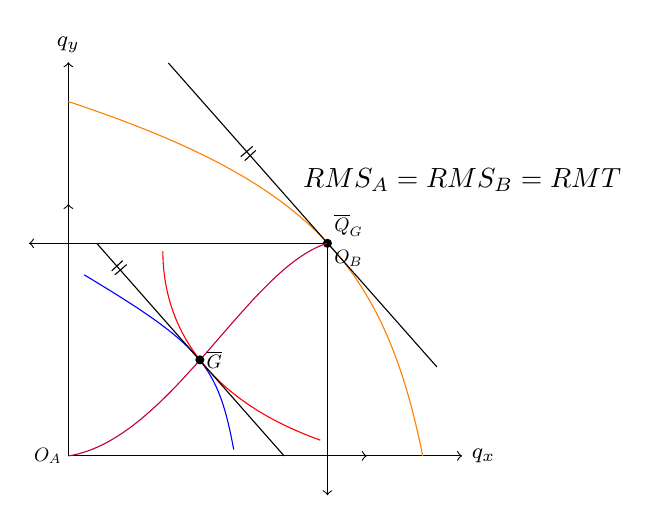
\begin{tikzpicture}
	% FPP
		% Ejes
			\draw[->] (10,0)-- (10,5) node[align=center, above] {\footnotesize $q_{y}$};
			\draw[->] (10,0) -- (15,0) node[align=center, right] {\footnotesize $q_{x}$};
		% Curva
			\draw [orange] (10,4.5) ..controls (13,3.5) and (14,2.5) .. (14.5,0);
			
	% Minicaja
		% Intersección
			\draw [<->] (9.5,2.7) -- (13.29,2.7) node [below right, scale=0.7] {$O_B$} -- (13.29,-0.5);
			\draw [<->] (10,3.2) -- (10,0) node [left, scale=0.7] {$O_A$} -- (13.79,0);
		% Puntos
			\draw[black, fill=black] (13.29,2.7) circle[radius=0.05] node [above right, scale=0.7] {$\overline{Q}_G$};
		% Curva de contrato
			\draw [purple] (10,0) ..controls (11.29,0.2) and (12.29,2.4) .. (13.29,2.7);
			\draw [blue] (10.2,2.3) ..  controls (11.7,1.4) and (11.9,1.15) .. (12.1,0.08);
			\draw [red] (11.2,2.6) ..  controls (11.2,1.6) and (11.8,0.7) .. (13.2,0.2);
		% Pendientes
			\draw (11.27,4.99) -- (14.68,1.13);
			\draw (10.36,2.7) -- (12.74,0);
		% Símbolo de paraleleas
			\draw (10.55,2.35) -- (10.69,2.48);
			\draw (10.59,2.3) -- (10.74,2.43);
			
			\draw (12.19,3.8) -- (12.34,3.93);
			\draw (12.24,3.75) -- (12.38,3.88);
		% 	Etqiueta
			\draw (15, 3.5) node {$RMS_A = RMS_B = RMT$};
		% Punto
			\draw[black, fill=black] (11.67,1.22) circle[radius=0.05] node [right, scale=0.7] {$\overline{G}$};
\end{tikzpicture}
		\end{center}
	\end{multicols}
\end{frame}
%------------------------------------------------
\begin{frame}{Si el panadero no fuese declarado responsable:}
	\begin{multicols}{2}
		\begin{itemize}
			\item $A$ = ganancia del médico, luego de compensar al panadero.
			\item $B$ = pérdida del panadero que será compensada por el médico
		\end{itemize}
		
		\begin{center}
			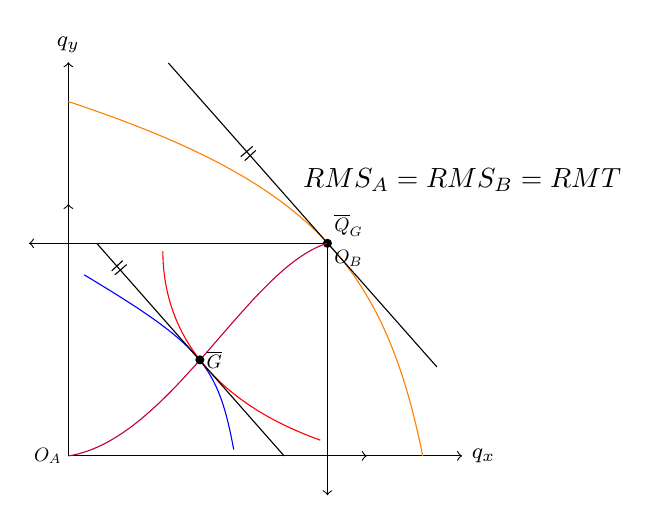
\begin{tikzpicture}
	% FPP
		% Ejes
			\draw[->] (10,0)-- (10,5) node[align=center, above] {\footnotesize $q_{y}$};
			\draw[->] (10,0) -- (15,0) node[align=center, right] {\footnotesize $q_{x}$};
		% Curva
			\draw [orange] (10,4.5) ..controls (13,3.5) and (14,2.5) .. (14.5,0);
			
	% Minicaja
		% Intersección
			\draw [<->] (9.5,2.7) -- (13.29,2.7) node [below right, scale=0.7] {$O_B$} -- (13.29,-0.5);
			\draw [<->] (10,3.2) -- (10,0) node [left, scale=0.7] {$O_A$} -- (13.79,0);
		% Puntos
			\draw[black, fill=black] (13.29,2.7) circle[radius=0.05] node [above right, scale=0.7] {$\overline{Q}_G$};
		% Curva de contrato
			\draw [purple] (10,0) ..controls (11.29,0.2) and (12.29,2.4) .. (13.29,2.7);
			\draw [blue] (10.2,2.3) ..  controls (11.7,1.4) and (11.9,1.15) .. (12.1,0.08);
			\draw [red] (11.2,2.6) ..  controls (11.2,1.6) and (11.8,0.7) .. (13.2,0.2);
		% Pendientes
			\draw (11.27,4.99) -- (14.68,1.13);
			\draw (10.36,2.7) -- (12.74,0);
		% Símbolo de paraleleas
			\draw (10.55,2.35) -- (10.69,2.48);
			\draw (10.59,2.3) -- (10.74,2.43);
			
			\draw (12.19,3.8) -- (12.34,3.93);
			\draw (12.24,3.75) -- (12.38,3.88);
		% 	Etqiueta
			\draw (15, 3.5) node {$RMS_A = RMS_B = RMT$};
		% Punto
			\draw[black, fill=black] (11.67,1.22) circle[radius=0.05] node [right, scale=0.7] {$\overline{G}$};
\end{tikzpicture}
		\end{center}
	\end{multicols}
\end{frame}
%------------------------------------------------
\begin{frame}{Si el panadero no fuese declarado responsable:}
	\begin{multicols}{2}
		\begin{itemize}
			\item Mientras $A >B$, el médico tiene incentivos para compensar, llegándose al óptimo.
			\item Más allá de $Q^S$, al médico no le conviene compensar
		\end{itemize}
		
		\begin{center}
			\begin{tikzpicture}[domain=5:10,
					tangent/.style={
						decoration={
							markings,% switch on markings
							mark=
							at position #1
							with
							{
								\coordinate (tangent point-\pgfkeysvalueof{/pgf/decoration/mark info/sequence number}) at (0pt,0pt);
								\coordinate (tangent unit vector-\pgfkeysvalueof{/pgf/decoration/mark info/sequence number}) at (1,0pt);
								\coordinate (tangent orthogonal unit vector-\pgfkeysvalueof{/pgf/decoration/mark info/sequence number}) at (0pt,1);
							}
						},
						postaction=decorate
					},
					use tangent/.style={
						shift=(tangent point-#1),
						x=(tangent unit vector-#1),
						y=(tangent orthogonal unit vector-#1)
					},
					use tangent/.default=1,
					scale=0.65
					]
	% Relleno
		\fill [pattern=crosshatch dots,pattern color=orange!60!white] (5,5) -- plot (\x, {sqrt(10-\x)/0.5 }) -- (5,0);\textbf{}
	% Ejes
		% Izquierda
			\draw[<->] (4,0) node[align=center, left, scale=0.8] {$-L$} -- (10,0) node[align=center, below] {\footnotesize $O_L$} -- (10,5) node[align=center, above, scale=0.8] {$q$};
		% Derecha
			\draw[<->] (5,5) node[align=center, above, scale=0.8] {$c$} -- (5,0) node[align=center, below, scale=0.8] {$O_R$} -- (11,0) node[align=center, right, scale=0.8] {$R$};
	% Curva
		\draw[color=orange,samples=1000, tangent=0.4] plot (\x, {sqrt(10-\x)/0.5 });
	% Punto - Tangente
		\filldraw[use tangent] (0,0) circle (2pt) node[align=center, above right, scale=0.8] {$M$};
	% Flechas
		\draw[<->] (5,-0.5) -- (7.5,-0.5) node[align=center, below, scale=0.8] {$\overline{L}$} -- (10,-0.5);
	% Curvas de indiferencia
		\draw [smooth,blue,thick] (6.3,5.5) to[out=299, in=161] (10.3,2.7);    
		\draw [smooth,blue,thick] (5.8,5) to[out=299, in=161] (9.8,2.2);
		\draw [smooth,blue,thick] (5.3,4.5) to[out=299, in=161] (9.3,1.7);
\end{tikzpicture}
		\end{center}
	\end{multicols}
\end{frame}
%------------------------------------------------
\begin{frame}{Si el panadero fuese declarado responsable:}
	\begin{multicols}{2}
		\begin{itemize}
			\item El médico maximiza beneficios en Q*.
			\item Si el médico recibe un poco de ruido
				\begin{itemize}
					\item Hay un pequeño perjuicio para él.
					\item Pero un gran beneficio para el panadero
				\end{itemize}
			\item Por tanto, el panadero tiene incentivos para compensar al médico, para poder producir.
		\end{itemize}
		
		\begin{center}
			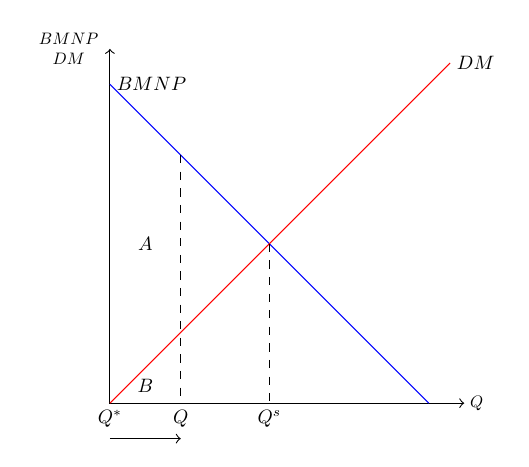
\begin{tikzpicture}[scale=0.9]
% Ejes
\draw[<->] (0,5)  node [text width=15mm,text centered, scale=0.6, left] {$BMNP$ $DM$}-- (0,0) -- (5,0) node [scale=0.6, right] {$Q$};

% Rectas
\draw[blue] (0,4.5) node [right, scale=0.7, black] {$BMNP$} -- (4.5,0);
\draw[red] (0,0)  node [below, scale=0.7, black] {$Q^\ast$} -- (4.8,4.8) node [right, scale=0.7, black] {$DM$};

% Rectas sombreadas
\draw[dashed] (1,3.5) -- (1,0)  node [below, scale=0.7, black] {$Q$};
\draw[dashed] (2.25, 2.25) -- (2.25,0) node [below, scale=0.7, black] {$Q^s$};

% A y B
\draw (0.5,2.25) node [scale=0.7, black] {$A$};
\draw (0.5,0.25) node [scale=0.7, black] {$B$};

% Flechas
\draw[->] (0,-0.5) -- (1,-0.5);
\end{tikzpicture}
		\end{center}
	\end{multicols}
\end{frame}
%------------------------------------------------
\begin{frame}{Si el panadero fuese declarado responsable:}
	\begin{multicols}{2}
		\begin{itemize}
			\item $A$ = ganancia del panadero, luego de compensar al médico.
			\item $B$ = pérdida del médico  que será compensada por el panadero.
			\item Mientras $A >B$, el panadero tiene incentivos para compensar, llegándose al óptimo.
			\item Más allá de $Q^s$, al panadero no le conviene  compensar.
		\end{itemize}
		
		\begin{center}
			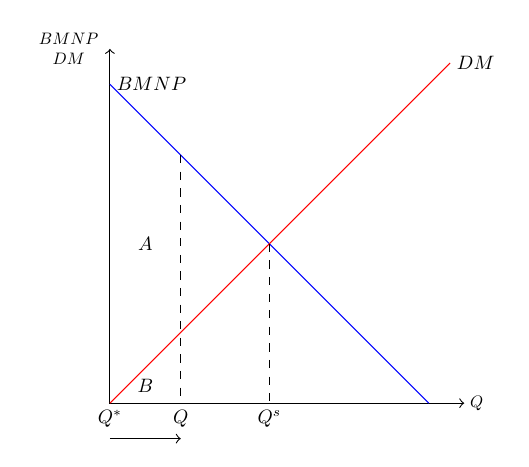
\begin{tikzpicture}[scale=0.9]
% Ejes
\draw[<->] (0,5)  node [text width=15mm,text centered, scale=0.6, left] {$BMNP$ $DM$}-- (0,0) -- (5,0) node [scale=0.6, right] {$Q$};

% Rectas
\draw[blue] (0,4.5) node [right, scale=0.7, black] {$BMNP$} -- (4.5,0);
\draw[red] (0,0)  node [below, scale=0.7, black] {$Q^\ast$} -- (4.8,4.8) node [right, scale=0.7, black] {$DM$};

% Rectas sombreadas
\draw[dashed] (1,3.5) -- (1,0)  node [below, scale=0.7, black] {$Q$};
\draw[dashed] (2.25, 2.25) -- (2.25,0) node [below, scale=0.7, black] {$Q^s$};

% A y B
\draw (0.5,2.25) node [scale=0.7, black] {$A$};
\draw (0.5,0.25) node [scale=0.7, black] {$B$};

% Flechas
\draw[->] (0,-0.5) -- (1,-0.5);
\end{tikzpicture}
		\end{center}
	\end{multicols}
\end{frame}
%------------------------------------------------
\begin{frame}{¿En qué casos si son relevantes las decisiones del Estado?}
	\begin{itemize}
		\item Cuando los costos de transacción son altos.
		\item Ejemplo: Aviones que hacen ruido en una zona residencial cercana al aeropuerto.
		\item En esos casos, la asignación de derechos que decida el Estado, debe basarse en un análisis económico para decidir la solución menos costosa.
	\end{itemize}
\end{frame}